198. \begin{figure}[ht!]
\center{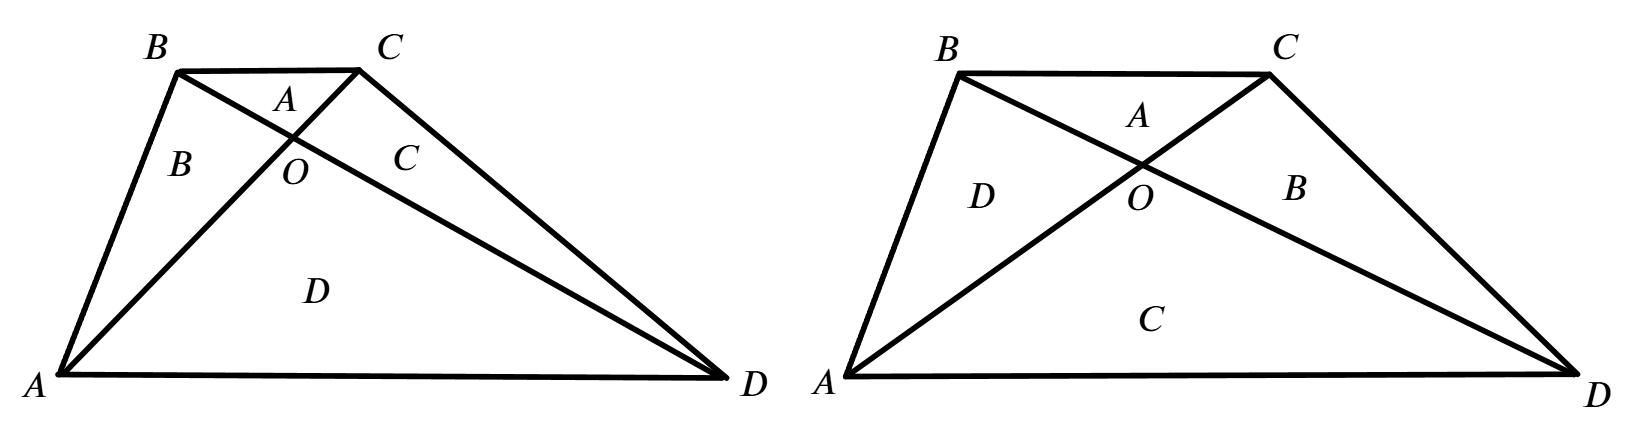
\includegraphics[scale=0.35]{g9-198.png}}
\end{figure}\\
Возможны два разных случая расположения площадей: площади $A$ и $D$ могут быть в трапеции соседними или противоположными.

Первый случай: они противоположны. Треугольники $AOD$ и $BOC$ подобны по двум углам, отношение их площадей равно $12:3=4,$ значит коэффициент подобия равен $\sqrt{4}=2$ и $AO:CO=2:1.$ У треугольников $ABO$ и $BCO$ общая высота из точки $B,$ значит их площади относятся как основания, к которым эта высота проведена, и $\cfrac{S_{\Delta ABO}}{S_{\Delta BOC}}=\cfrac{AO}{CO}=2:1,$ откуда $S_{\Delta ABO}=2\cdot3=6,$ аналогично и $S_{\Delta CBO}=6.$ Поэтому в данном случае площадь трапеции $ABCD$ равна $3+12+6+6=27.$

Второй случай: они соседние. Тогда аналогично первому случаю имеем соотношение $\cfrac{AO}{OC}=\cfrac{S_{\Delta ABO}}{S_{\Delta BOC}}=12:3=4,$ а значит треугольники $AOD$ и $BOC$ подобны с коэффициентом 4 и $S_{\Delta AOD}=16S_{\Delta BOC}=16\cdot3=48.$ Так как $OD:BO=4,$ то и $S_{\Delta COD}=3\cdot4=12,$ а значит площадь всей трапеции $ABCD$ равна $3+48+12+12=75.$\\
